\chapter{バッチSWMH}
前章で説明したSWMHでは,データストリームに毎時刻要素が1つだけ到着することを仮定したが,現実のデータストリームでは,1度に複数個の要素が到着することも普通である.そこで,そのような場合にSWMHを拡張することを目指す,本章では,データストリームに毎時刻$c$個の要素が到着するモデルを想定する.
%私たちは,4節で紹介したSWMHをスライディングに毎時刻複数個の要素が出入りする場合に対応するMinlist更新アルゴリズムであるバッチSWMHを開発した.


\section{自明な手法}
データストリームに毎時刻$c$個の要素が到着するモデルにおいての自明な手法は,4章で説明したSWMHを$c$回適応する手法である.つまり,スライディングウインドウが$c$回ずれる事象を,スライディングウインドウが1つずれる事が$c$回繰り返されると判断して,SWMHを$c$回適用する,1回SWMHを適用する度にMinlistが1回適用されるので,1時刻あたり$c$回Minlistをスキャンすることになる.


\begin{figure}[H]
  \centering
  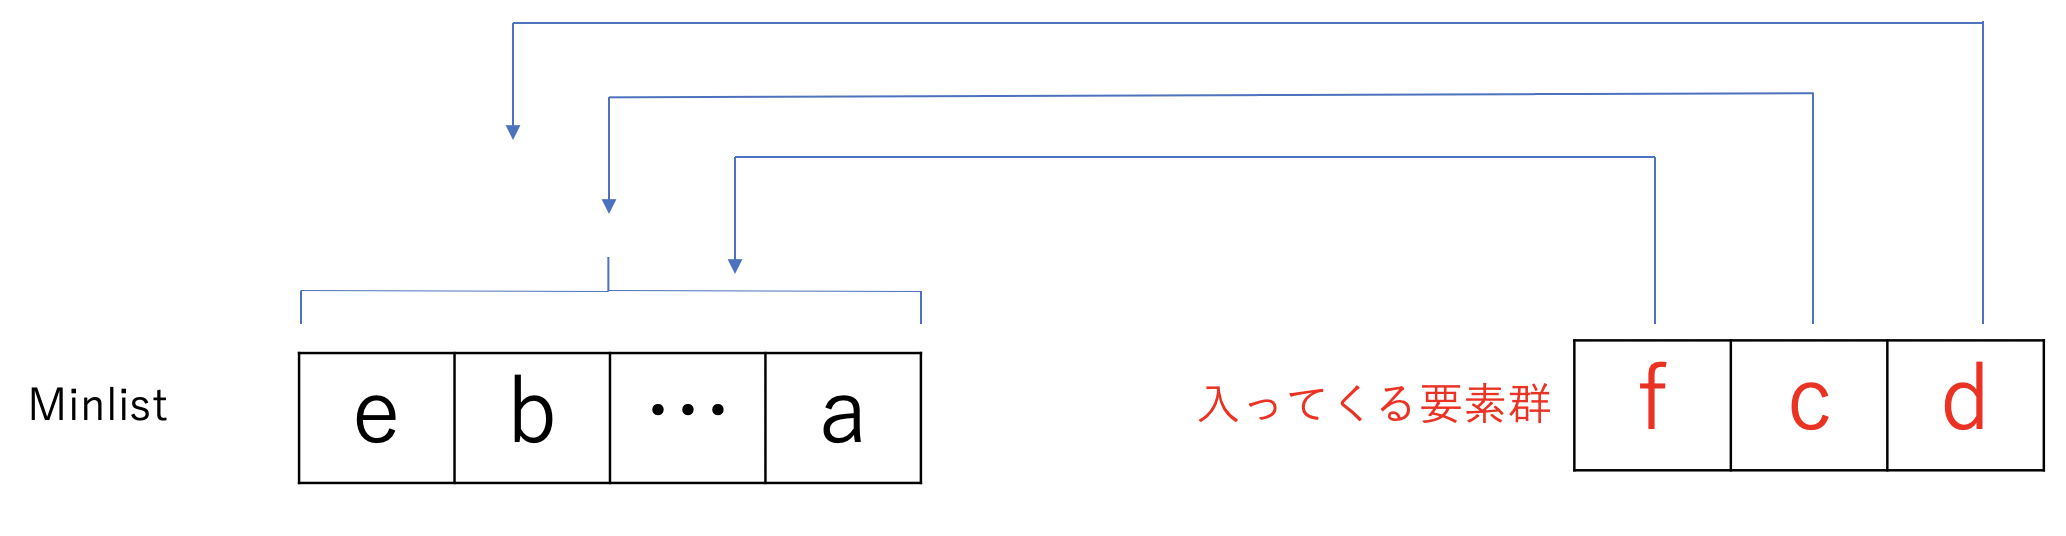
\includegraphics[width=15cm]{6_1.png}
    \caption{Minlistの更新}
\end{figure}

\section{バッチSWMHのアルゴリズム}
本章ではMinlistを$c$回スキャンせず1回だけスキャンするバッチSWMHを提案する.
バッチSWMHのアルゴリズムでは,ウインドウから要素が出ていく場合と入ってくる場合に処理を分けて考える.ウインドウにc個の要素が出入りする場合,ウインドウから出ていく要素群を$E_{t-w/c+1} = $\{$e^1_{t-w/c+1},e^2_{t-w/c+1},...,e^c_{t-w/c+1}$\},入ってくる要素群を$E_{t} = $\{$e^1_t,e^2_t,...,e^c_t$\}とする.

\subsection{要素群$E_{t-w/c+1}$が出ていく処理}
バッチSWMHの$E_{t-w/c+1}$が出ていく処理では,4.2.1節のSWMHのウインドウから要素が出ていく時に対する処理と同じように場合分けをして処理を行う.Minlist 内で最小割り当て値となる要素$\alpha$のアルファベットを$x$と記述する.

\noindent (Case1):Minlistの先頭要素の時刻が$t-w/c+1$ならばMinlistの先頭要素をデキューする.さらに,Minlistの要素が$t-w/c+1$と違う時刻要素が出てくるまでMinlistをスキャンし,$t-w/c+1$と同じ時刻を持つ要素を削除する.この時,削除される要素が$\alpha$と同じアルファベット$x$を持つ場合,新たな最小割り当て値となる要素をMinlistから探索して更新する.Minlistは割り当て値順にソートされていないので,この操作はMinlistの全要素のスキャンを伴う.

\noindent (Case2):Minlistの先頭時刻が$t-w/c+1$でない場合,Minlistからのデキューは不要である.不要である理由は,4.2.1節で説明した理由と同じである.


\subsection{要素群$E_t$が入ってくる処理}
Minlistに$E_t$が入ってくる処理では,以下の3つの手順で行う.
\begin{itemize}
\item $E_t$から代表アルファベットの選択
\item 代表アルファベットと比較して,Minlistをスキャン
\item Minlistへ$E_t$を追加

代表アルファベットとは,$E_t$の中で割り当て値が最小のアルファベット$x$と$E_t$の中でスライディングウインドウ内の多重度最大のアルファベット$y$である.

そして,Minlistのスキャンでは,$E_t$内の要素と同じラベルの要素の削除と違うラベルの削除の2つの処理を行う.Minlistの要素を$\lambda$とする.
(1) $E_t$内の要素と同じラベルの要素の削除

同じアルファベットを消すために,従来の手法では,$\lambda$に対して,$E_t$全体をスキャンし,同じアルファベットが複数存在するか確認する必要があった.しかし,私たちは先に保持させたヒストグラムの情報の1つである時刻を用いて,ヒストグラムの最後尾に入っている要素の時刻と$l(\lambda)$の時刻を比較することで,同じアルファベットの中で一番最後尾の要素のみを残し,ほかの要素を削除することができる.

 (2)$E_t$内の要素と違うラベルの要素の削除
$E_t$の中で,$x$,$y$の2つのアルファベットを用いてスキャンを行なっていく.Minlist内の要素$\lambda$の入ってきた時刻$t_\lambda$とし,$t_\lambda$よりあとに到着した$x$, $y$の個数$n_x$,$n_y$とする.時刻に応じて,$x$,$y$のうち小さい割り当て値を持つアルファベットの割り当て値を用いて,Minlistから将来の割り当て値の上限を上回る要素を削除していく.

\begin{quote}
$\pi_{{\rm min}} = {\rm min}(\pi(x_{n_x}),\pi(y_{n_y}))$ \\
 {\bf if} ($\pi_{{\rm min}}<\pi(l(\lambda))$)  Minlistから $\lambda$を削除\\
\end{quote}
% まず,$E_t$の要素すべてヒストグラムに追加する.始めにヒストグラムに追加することを利用して,以下の3つの手順で処理を行う.


%\subsubsection{ \scalebox{1.2}{手順1:要素群の更新と代表アルファベットの選択}}
%$E_t$を後ろからスキャンし,将来最小値になり得ない要素の削除と,Minlistをスキャンする際の基準アルファベットの選択を行う.基準アルファベットとは,$E_t$の中で割り当て値が最小のアルファベット$x$と$E_t$の中でスライディングウインドウ内の多重度最大のアルファベット$y$である.
%$c$個の要素群が入ってくることに対して,その中の1つのアルファベットだけでMinlistをスキャンより,2つのアルファベットを使う方が割り当て値の変化により対応でき,Minlistを短く保つことにつなるために,基準アルファベットを2つ選択する.
%スキャンされる側の$E_t$内の要素を$e^z_t (1 \le z<c)$,$E_t$の一番最後尾の要素$e^c_t$のラベルのアルファベットを $x = l(e^c_t)$,$y = l(e^c_t)$として,後ろから順に以下の処理を行なっていく.

%(1) $e^z_t$と同じアルファベットが$E_t$内に複数存在するか確認

 %$e^z_t$と同じアルファベットを消すために,従来の手法では,$E_t$全体をスキャンし,同じアルファベットが複数存在するか確認する必要があるため,$O(c)$の時間を要する.しかし,私たちは先に保持させたヒストグラムの情報の1つである時刻を用いて,ヒストグラムの最後尾に入っている要素の時刻と$e^z_t$の時刻を比較することで,同じアルファベットの中で一番最後尾の要素のみを残し,ほかの要素を削除することができる.
 
 %(2)違うアルファベットの中で必要ない要素の削除とx,yの更新
 %$\pi(e^z_t)$より$\pi(x)$が大きい場合, $e^z_t$を削除し,小さい場合$x$を更新する,さらに,$e^z_t$のアルファベットが$E_t$内でヒストグラム最大の場合,$y$を更新する.

%\begin{quote}
%{\bf if} ( $\pi(x) \le \pi(e^z_t)$ )\{ \\
%\hspace*{1cm} $e^z_t$を$E_t$から削除する.\\
%\}
%{\bf else}  $x = \l(e^z_t)$  \\

%{\bf if} ( ${ \rm histgram}(y).{\rm size} < { \rm histgram}(\l(e^z_t)).{\rm size}$ ) $y = \l(e^z_t)$

%\end{quote}


%\begin{equation}
 %\label{eq:5_2}
%x = \l(e^a_t) \; \; \; (1\le a \le c-1)
%\end{equation}\

%(3)入ってきた要素群$E_t$から将来最小値になり得る要素のみを残した要素群$E'_t$として保持する.


%\subsubsection{ \scalebox{1.2}{手順2:Minlistのスキャン}}
%手順2では,Minlist内で手順1と同じように$E'_t$の要素のアルファベットと同じ要素の削除と,将来最小値になり得ないアルファベットを持つ要素の削除を行なっていく.同じアルファベットの要素の削除は,手順1の方法により,ヒストグラムを利用して削除していく.
%将来最小値になり得ないアルファベットを持つ要素の削除するために,$E_t$の中で,$x$,$y$の2つのアルファベットを用いてスキャンを行なっていく.Minlist内の要素$\lambda$の入ってきた時刻$t_\lambda$とし,$t_\lambda$よりあとに到着した$x$, $y$の個数$n_x$,$n_y$とする.時刻に応じて,$x$,$y$のうち小さい割り当て値を持つアルファベットの割り当て値を用いて,Minlistから将来の割り当て値の上限を上回る要素を削除していく.

%\begin{quote}
%$\pi_{{\rm min}} = {\rm min}(\pi(x_{n_x}),\pi(y_{n_y}))$ \\
 %{\bf if} ($\pi_{{\rm min}}<\pi(l(\lambda))$)  Minlistから $\lambda$を削除\\
%\end{quote}



\subsubsection{ \scalebox{1.2}{手順3:Minlistへの追加}}
最小値となり得ない要素を削除したMinlistに対して,$E'_t$を追加する.

%\begin{quote}
%{\bf if} ($   \pi(y_{n_x}) \le \pi(y_{n_y})$)\{ \\
%\hspace*{1cm} {\bf if} ($\pi(a_{i+1})>\pi'(a_i)$) $\pi'(a_{i+1})=\pi'(a_i)$ \\
%\hspace*{1cm} {\bf else} $\pi'(a_{i+1})=\pi(a_{i+1})$ \\
%\}